% !TeX spellcheck = en_US


\chapter{Conclusion}


\section{Future Work}
\begin{frame}{Future Work}
    \begin{itemize}
        \item Testing of the whisker control system with the Franka Emika Panda robotic arm
        \item Addition of more whiskers to each side of the platform
        \item Active exploration of unstructured environments
        \item SLAM for navigation in cluttered environments
        \item Integration of the whiskers into the robotic rat
    \end{itemize}
\end{frame}


\section{Summary}
\begin{columns}[T,onlytextwidth]
    \begin{column}[T]{0.6\textwidth}
        \begin{enumerate}
            \item A \textbf{whisker array platform} for active tactile exploration was designed and assembled
            \item Control algorithms were implemented for:
            \begin{itemize}
                \item Contour reconstruction
                \item \textbf{Object retrieval}
                \item \textbf{Navigation in tunnels}
            \end{itemize}
            \item A \textbf{test framework with physics simulation} was developed for the whisker control system
            \item A \textbf{system infrastructure} was developed for real-time sensor data visualization and evaluation
        \end{enumerate}
    \end{column}
    \begin{column}[T]{0.4\textwidth}
        \begin{figure}[H]
            \centering
            \captionsetup{justification=centering}
            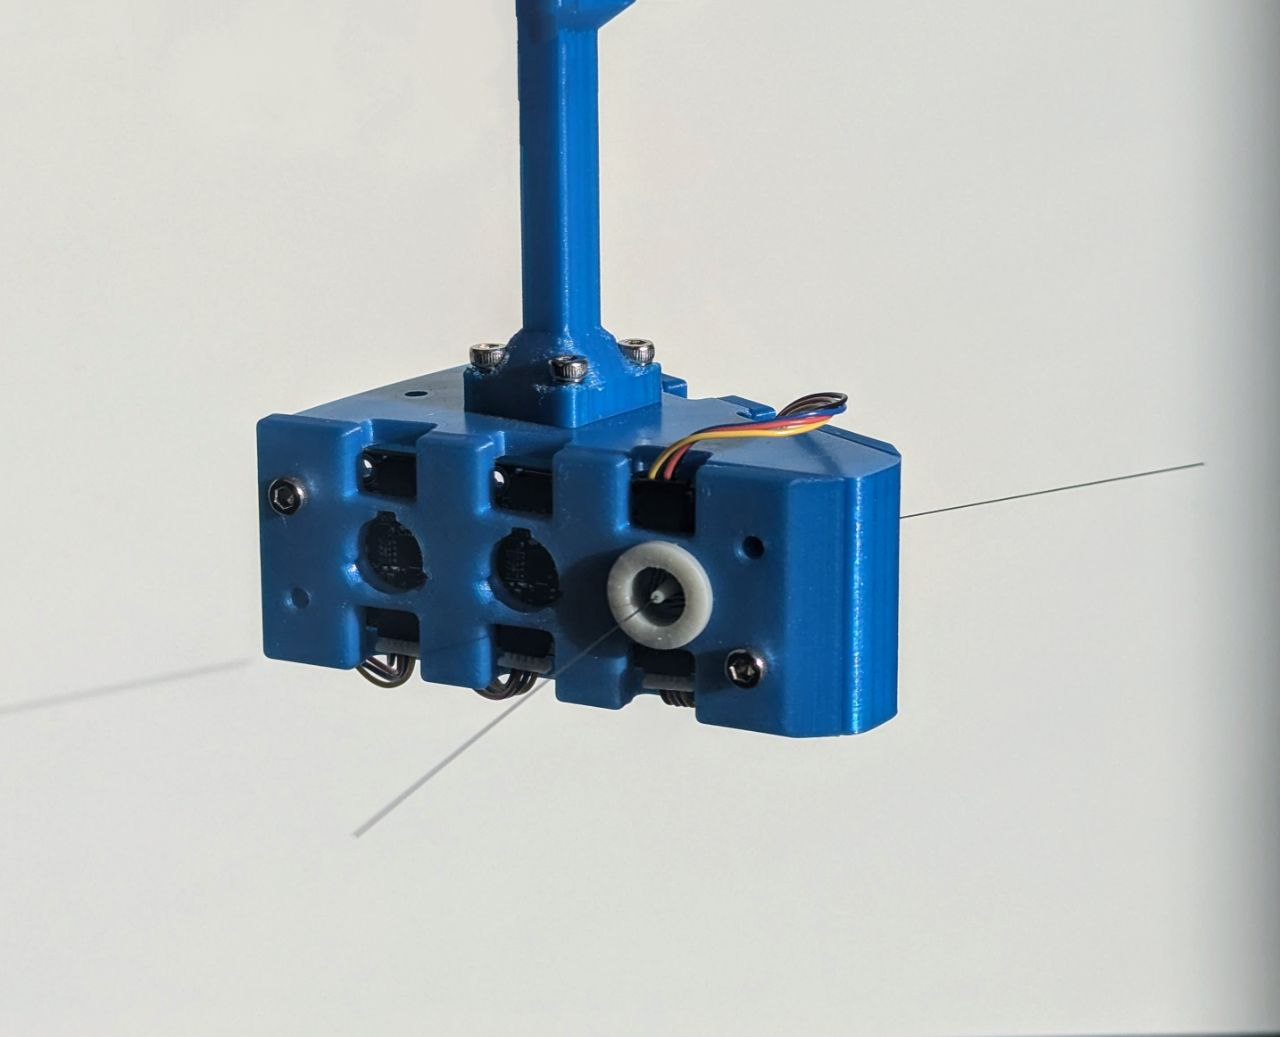
\includegraphics[width=0.7\textwidth]{figures/platform-two-whiskers}
            \caption{Platform with left and right whiskers}
        \end{figure}
        \vskip-1cm
        \begin{figure}[H]
            \centering
            \captionsetup{justification=centering}
            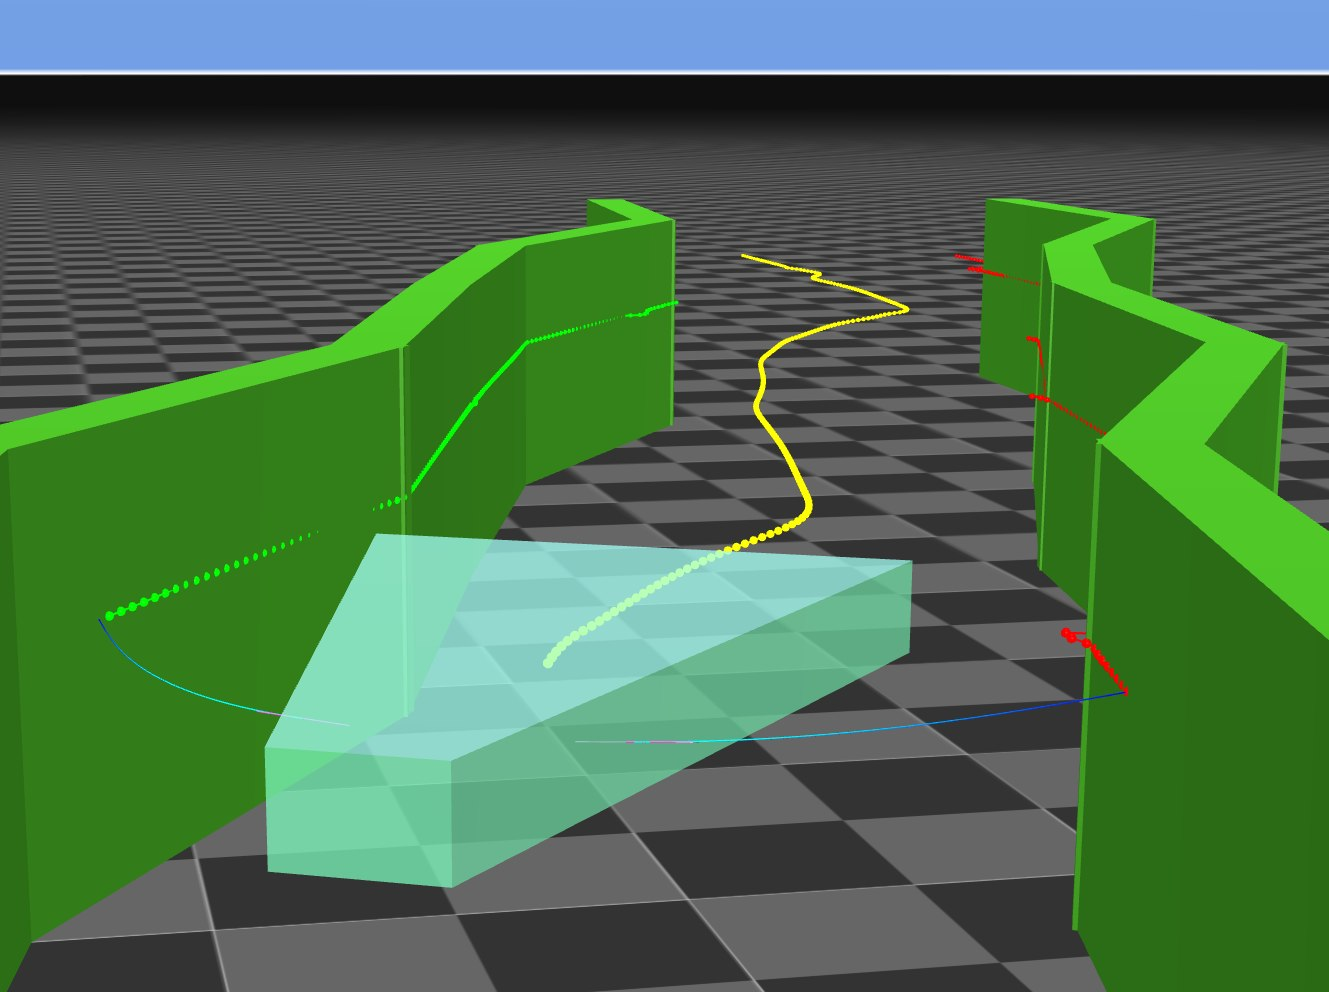
\includegraphics[width=0.7\textwidth]{figures/platform-in-tunnel}
            \caption{Simulation: platform navigating in a tunnel}
        \end{figure}
    \end{column}
\end{columns}